\documentclass{standalone}

\usepackage{../thesis}

\usepackage[americaninductors]{circuitikz}
\usetikzlibrary{decorations.pathmorphing}
\usepackage{pgfplots} % drawing plots right here in this file!
\pgfplotsset{compat=1.9} % latest stable release

\begin{document}

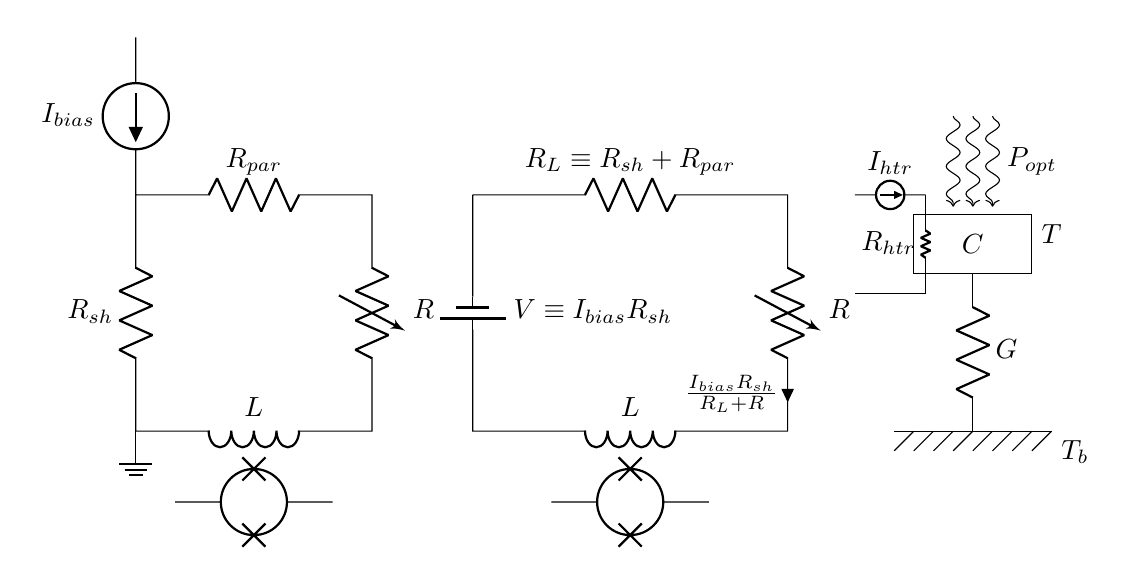
\begin{tikzpicture}
\matrix{
	\draw
	(0,5) to[american current source, l_=$I_{bias}$] (0,3)
	      to[R, l=$R_{par}$] (3,3)
	      to[vR, l=$R$] (3,0)
	      to[L, l_=$L$] (0,0)
	      to[R, l=$R_{sh}$] (0,3)
	(0,0) node[ground] {}
	(0.5, -0.9) to[squid] (2.5,-0.9);
 	& 
	\draw
	(0,3) to[R, l={$R_L \equiv R_{sh} + R_{par}$}] (4,3)
	      to[vR, l=$R$, i_=$\frac{I_{bias} R_{sh}}{R_L + R}$] (4,0)
	      to[L, l_=$L$] (0,0)
	      to[battery1, l_=$V \equiv I_{bias} R_{sh}$] (0,3)
	(1.0, -0.9) to[squid] (3.0,-0.90);
	&
    % First the light falling on the bolometer
	\draw [->] decorate [decoration={snake}] {(-0.25,4.0) -> (-0.25,2.85)};
	\draw [->] decorate [decoration={snake}] {( 0.00,4.0) -> ( 0.00,2.85)};
	\draw [->] decorate [decoration={snake}] {( 0.25,4.0) -> ( 0.25,2.85)};
	\draw (0.75, 3.425) node {$P_{opt}$};
    
    % Now the thermal link and heat capacity
    \draw (0,2) to[R, l=$G$] (0,0);
    \draw (-0.75,2) rectangle (0.75,2.75) node[midway] {$C$} node[below right] {$T$};
    
    % Now the temperature bath
    \draw (-1,0) -- (1,0) node[below right] {$T_b$};
    \draw (-1.00,-0.25) -- (-0.75,0);
    \draw (-0.75,-0.25) -- (-0.50,0);
    \draw (-0.50,-0.25) -- (-0.25,0);
    \draw (-0.25,-0.25) -- (-0.00,0);
    \draw ( 0.00,-0.25) -- ( 0.25,0);
    \draw ( 0.25,-0.25) -- ( 0.50,0);
    \draw ( 0.50,-0.25) -- ( 0.75,0);
    \draw ( 0.75,-0.25) -- ( 1.00,0);
    
    % now the heater resistor
    \draw (-1.5,3.0) to[american current source, l^=$I_{htr}$, bipoles/length=0.6cm] (-0.6,3.0);
    \draw (-0.6,3.0) to[R, l_=$R_{htr}$, bipoles/length=0.4cm] (-0.6, 1.75) to (-1.5,1.75);
    \\
	};
\end{tikzpicture}

\end{document}
